\section{Introduction}
\label{sec:intro}

Continual learning methods limit forgetting by reusing old examples or restricting how far parameters move from a previous solution~\citep{rolnick2018,kirkpatrick2016}. Their retention depends on the stream: an old task may return after one update or after a long run on another task. A frequency-domain view asks whether tuning for one timescale necessarily hurts another. If the total log-gain were fixed at a matched final fit, a retention method could move sensitivity across frequencies but could not lower it throughout the spectrum.

We test this prediction by modulating the old-task fraction around a fixed mixture. In \cref{fig:spectra}, increasing only the learning rate increases the old-task loss response at every sampled frequency. No compensating reduction appears. A lock-in calibration with known harmonics and a separate linearized transfer recover the expected responses (\cref{sec:calibration}); the discrepancy is with the invariance claim, not with the estimator.

Different terminal fits could explain gain differences between replay and consolidation. The two gradient-descent arms remove that explanation: they use the same teachers and initialization, take the same number of steps, and reach the same unforced predictor, with identical per-task losses. The rate change alone produces a 1.782 log-unit area gap. Across all four arms, the range is 46.3\% of the mean absolute area, beyond the specified 20\% rejection threshold (\cref{tab:main,tab:ablations}).

The distinction is between a closed-loop sensitivity with a fixed leading coefficient and an input-to-loss transfer whose leading coefficient can change. The one-step loss response depends on the learning rate, the operating point, and how the update uses the incoming mix. We identify that coefficient and the out-of-circle zeros as the relevant terms (\cref{prop:jensen}). The resulting conditional identity describes the local response; it does not constrain absolute forgetting or guarantee a tradeoff in stochastic training.

\begin{figure}[!t]
  \centering
  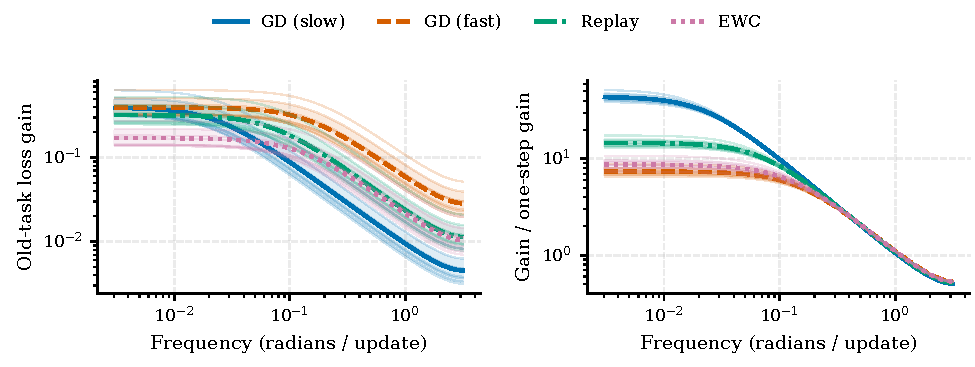
\includegraphics[width=\textwidth]{spectra.pdf}
  \caption{\textbf{The learning-rate change raises raw gain throughout the sampled band.}
  Left: gain from old-task fraction to old-task squared loss at amplitude 0.01 over 55 frequencies up to Nyquist. Right: gain divided by the absolute one-step gain for each arm and seed. Heavy lines are geometric means across eight paired seeds; bands are pointwise 95\% Student-\(t\) intervals on log-gain; faint lines are individual seeds. GD is gradient descent; EWC is elastic weight consolidation.}
  \label{fig:spectra}
\end{figure}

\section{Problem statement}
\label{sec:problem}

Let \(A\) be an old task initially solved by the learner, and \(B\) a conflicting new task. At step \(t\), let \(u_t\in[0,1]\) denote the incoming old-task fraction.

The learner scores its current parameters on \(A\), then updates using the mixture and any method-specific memory. We drive \(u_t=\tfrac12+\alpha\cos(\omega t)\), with amplitude \(\alpha>0\) and frequency \(\omega\) in radians per update. The old-task loss is \(\ell_A(\theta_t)\), where \(\theta_t\) denotes the parameters before update \(t\). The transfer \(S\) maps a small perturbation of \(u_t\) to a perturbation of this loss at the unforced operating point. The measured gain is the fundamental harmonic amplitude of the settled loss divided by \(\alpha\).

We test the mean log-area
\begin{equation}
  \mathcal{I}=\frac{1}{\pi}\int_0^\pi \log |S(e^{i\omega})|\,d\omega.
  \label{eq:area}
\end{equation}
The raw claim predicts that the range of \(\mathcal I\) is at most 20\% of its mean absolute value at matched terminal joint accuracy. This threshold is a decision rule in fixed loss units, not a scale-invariant physical constant: multiplying the loss by a common factor shifts each area by the same log constant. We therefore report the area difference and its exponential, the ratio of geometric-mean gains. The area weights frequencies uniformly in \(\omega\), not uniformly on the logarithmic axis used to draw \cref{fig:spectra}.

The output is loss, not classification accuracy: at a point where the gradient of old-task loss vanishes, the first-order loss transfer vanishes even if the predictor moves. We measure retention separately as terminal sign accuracy and the mean increase in old-task loss from the initial fit. This separates steady operating-point degradation from the response to a small change in the mix. Cyclic forgetting bounds and tracking analyses answer different questions: they bound a loss after repeated task exposures or track a moving optimum, rather than integrating the old-task loss response around a fixed mixture.
